% !TEX root =  ../main.tex
\section{MostlySpread}

\subsection{Definition}

\subsubsection{Signature} \cstr{mostlySpread(s : set<VM>, n : number)}

\begin{itemize}
\item \cstr{s} : a non-empty set of virtual machines for a meaningful constraint
\item \cstr{n}: a positive number, inferior to the number of virtual machines in \cstr{s}
\end{itemize}

The \cstr{mostlySpread} constraint ensures the running virtual machines in \cstr{s} will be running
on at least \cstr{n} distinct servers.

\classification{mostlySpread}{application administrator}{VM placement}{VM-to-VM placement,Fault tolerance, Partitioning}


\subsubsection{Usage}

The \cstr{mostlySpread} constraint may be used by an application administrator to provide to a replicated service, fault tolerance to hardware failures. By hosting replaces on distinct servers, the service will  be available while at least one server is still online. When the number of replicas is important, it is however difficult to have a large amount of different servers. Furthermore, the chances of having all the hosting hervers but one failing simultaneously decrease when the number of replicas increases. It is then tolerable to use a number of servers that is smaller to the number of replicas.
The application administrator can then use one \cstr{mostlySpread}�constraint to indicate
the minimum number of distinct servers that must be used to host the replicas.

\subsubsection{Example}

Figure~\ref{fig: mostlySpread} depicts a sample reconfiguration between a source and a destination
configuration. In this example, the following \cstr{mostlySpread} constraints were considered:


\begin{reconfiguration}
\centering
\begin{minipage}[b]{0.40\textwidth}
\begin{lstlisting}
N1: VM1 VM2
N2: VM5
N3: VM3
\end{lstlisting}
\end{minipage}
\begin{minipage}[b]{2cm}
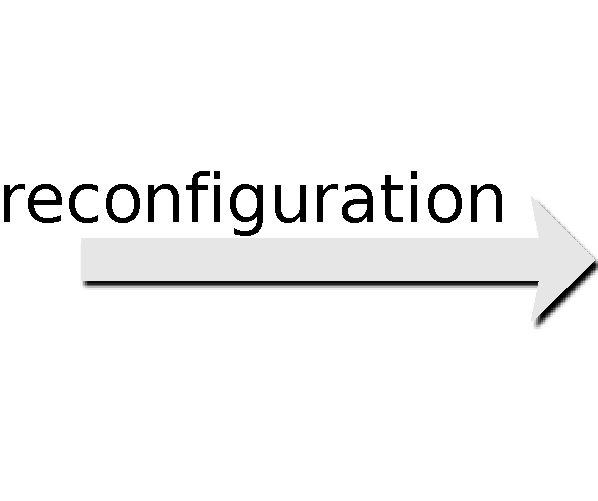
\includegraphics[width=2cm]{img/arrow_reconfiguration}
\end{minipage}
\begin{minipage}[b]{0.40\textwidth}
\begin{lstlisting}
N1: VM1 VM6
N2: VM2
N3: VM3 VM5
\end{lstlisting}
\end{minipage}
\caption{A reconfiguration motivated by \cstr{mostlySpread} constraints.}\label{fig: mostlySpread}
\end{reconfiguration}

\begin{itemize}

\item \cstr{mostlySpread(\{VM1, VM2, VM5\}, 2)}. This constraint was satisfied in the sour\-ce configuration as all the VM were running on  2 distinct servers. The constraint is still satisfied in the destination configuration as all the VMs are running on 3 distinct servers.

\item \cstr{mostlySpread(\{VM1,VM2\}, 1)}. This constraint was not satisfied in the source configuration as the VMs where running on \cstr{N1}. The relocation of \cstr{VM2} to \cstr{N3} fixed this violation.

\end{itemize}

\subsection{See also}

\subsubsection{Related Constraints}
\begin{itemize}
\item \cstrref{spread}: a constraint that guarantees the VMs will never overlap on a same server, even during the reconfiguration process.
\item \cstrref{lazySpread}: a constraint similar to \cstr{mostlySpread} but that guarantee every VMs are running on distinct servers.
\end{itemize}

\printListOfInheritance{mostlySpread}
